%!TEX root = main.tex

There has recently been a sharp growth in the number of knowledge graph datasets that are made available in the RDF (Resource Description Framework)\footnote{\url{https://www.w3.org/RDF}} data model.
Examples include knowledge graphs that cover a broad set of domains such as DBpedia~\cite{lehmann2015dbpedia}, YAGO~\cite{yago2}, Wikidata~\cite{vrandecic12wikidata},
and BabelNet~\cite{Navigli:2012:BAC:2397213.2397579}, 
as well as specialized graphs for specific domains like %social media networks,
product graphs for e-commerce~\cite{Dong:2018:CIB:3219819.3219938}, biomedical information networks~\cite{belleau2008bio2rdf}, %, ruttenberg2009life}.
and bibliographic datasets~\cite{mccallum2000automating, giles1998citeseer}.
The rich information and semantic structure of knowledge graphs makes them 
useful in many machine learning applications~\cite{davis1993knowledge},
such as recommender systems~\cite{jenatton2012latent},
virtual assistants, and question answering systems~\cite{west2014knowledge}.
Recently, many machine learning algorithms have been developed specifically for %analyzing
knowledge graphs,
especially in the sub-field of \textit{relational learning}, which is dedicated to learning from
the 
relations between entities in a knowledge graph~\cite{nickel2015review, nguyen2017overview, wang2018multi}.

RDF is widely used to publish knowledge graphs as it provides a powerful abstraction for representing heterogeneous, incomplete, sparse, and potentially noisy knowledge graphs. RDF is supported by a rich ecosystem of data management systems and tools that has evolved over the years.
This ecosystem includes standard serialization formats, parsing and processing libraries,
and most notably RDF database management systems (a.k.a. \textit{RDF engines} or \textit{triple stores}) that support \sparql,\footnote{\url{https://www.w3.org/TR/sparql11-query}}
the W3C standard query language for RDF data.
%These systems are also known as \textit{triple stores}. 
Examples of these systems include
OpenLink Virtuoso,\footnote{\url{https://virtuoso.openlinksw.com}}
Apache Jena,\footnote{\url{https://jena.apache.org}}
and
managed services such as
Amazon Neptune.\footnote{\url{https://aws.amazon.com/neptune}}

\textit{However, we make the observation that none of the publicly available machine learning or relational learning tools for knowledge graphs that we are aware of uses \sparql
%to query knowledge graphs in RDF database systems
to explore and extract datasets from knowledge graphs stored in RDF database systems.} 
 This, despite the obvious advantage of using a database system such as data independence, declarative querying, and efficient and scalable query processing.
For example, we investigated all the prominent recent open source relational learning implementations,
and we found that they all rely on ad-hoc scripts to process very small knowledge graphs and prepare the necessary datasets for learning.
This observation applies to the implementations of published state-of-the-art embedding models, e.g., scikit-kge~\cite{nickel2016holographic, nickel2011three},\footnote{\url{https://github.com/mnick/scikit-kge}}
and also holds for the recent Python libraries that are currently used as standard implementations for training and benchmarking knowledge graph embeddings, e.g.,
Ampligraph~\cite{ampligraph}, OpenKE~\cite{han2018openke}, and PyKEEN~\cite{ali2020pykeen}.
These scripts are limited in performance, which slows down data preparation and leaves the challenges of applying embedding models on the scale of real knowledge graphs unexplored. 

We posit that machine learning tools do not use RDF engines due to an ``impedance mismatch.''
Specifically, typical machine learning software stacks are based on data in \textit{tabular format} and the split-apply-combine paradigm~\cite{Wickham_2011}.
An example tabular format is the highly popular \textit{dataframes},
supported by libraries in several languages such as Python and R
(e.g., the pandas\footnote{\url{https://pandas.pydata.org}}
and scikit-learn libraries in Python),
and by systems such as Apache Spark~\cite{apacheSpark}.
Thus, the first step in most machine learning pipelines
(including relational learning) 
is a data preparation step that
explores the knowledge graph,
identifies the required data,
extracts this data from the graph,
efficiently processes and cleans the extracted data,
and returns it in a table.
% ;
% machine learning tools cannot work directly on data in an RDF database system.
Identifying and extracting this refined data from a knowledge graph requires efficient and flexible \textit{graph traversal} functionality. \sparql is a declarative pattern matching query language
%built on the RDF data model which is 
designed for distributed data integration with unique identifiers 
%exchange and publishing of data rather than efficient processing and navigation in the graph. 
rather than navigation~\cite{Matsumoto2018MappingRG}. 
Hence, while \sparql has the expressive power to process and extract data into tables, machine learning tools do not use it  since it lacks the required flexibility and ease of use of \textit{navigational} interfaces.
%learning and graph analysis algorithms don't use 
%as it lacks the \textit{navigation} interface naturally required to process and query graphs. 

In this paper, we introduce \textit{\rdfframes},
%(name hidden for double-blind reviewing),
%\footnote{Name hidden for double-blind reviewing.} 
a framework that bridges the gap between machine learning tools and RDF engines.
%database systems.
%Specifically,
\rdfframes is designed to support the data preparation step.
It defines a user API consisting of two type of operators: navigational operators that explore an RDF graph and extract data from it based on a graph traversal paradigm, and relational operators for processing this data into refined clean datasets for machine learning applications.
%\rdfframes defines an API consisting of this set of operators, 
The sequence of operators called by the user represents a logical description of the required dataset.
%defines a logical representation of the dataset required
\rdfframes translates this description to a corresponding \sparql query, executes it 
%against
on an RDF engine,
%database system,
and returns the results as a table.
%and the user calls these operators to define the data that is required from the graph.
%processes the 
%navigational 

In principle, the \rdfframes operators can be implemented in any programming language and can return data in any tabular format.
However, concretely, our current implementation of \rdfframes is a Python library that returns data as dataframes of the popular pandas 
%Python 
library
so that further processing can leverage
%be done using the 
the richness
% features 
of the PyData ecosystem.
\rdfframes is available as open source\footnote{\url{https://github.com/qcri/rdfframes}}
%(link hidden for double-blind reviewing)
%\footnote{Link hidden for double-blind reviewing.}
and via the Python 
pip installer. It is implemented in 6,525 lines of code, and was demonstrated in~\cite{rdfframes-demo}.

\vspace{4pt}
\noindent
\textbf{Motivating Example.}
We illustrate the end-to-end operation of \rdfframes through an example.
Assume the DBpedia knowledge graph is stored in an RDF engine,
and consider a machine learning practitioner who wants 
use DBpedia
to study
prolific American actors (defined as those who have starred in 50 or more movies).
Let us say that the practitioner wants to see
the movies these actors starred in
and the Academy Awards won by any of them.
Listing~\ref{lst:motivating_code} shows Python code using the \rdfframes API that prepares a dataframe with the
data required for this task.
It is important to note that this code is a \textit{logical description} of the dataframe and \textit{does not cause a query to be generated or data to be retrieved from the RDF engine.}
At the end of a sequence of calls such as these, the user calls a special \texttt{execute}
function that causes a \sparql query to be generated and executed on the engine, and the results to be returned in a dataframe.

The first statement of the code creates a two-column
\rdfframe with 
the URIs (Universal Resource Identifiers) of
all movies and all the actors who starred in them.
The second statement navigates from the actor column in this 
\rdfframe to get the birth place of each actor and uses a filter
to keep only American actors.
Next, the code finds all American actors who have starred
in 50 or more movies (prolific actors).
This requires grouping and aggregation, as well as a filter 
on the aggregate value.
The final step is to navigate from the actor column in the prolific actors 
\rdfframe to get the actor's Academy Awards (if available).
The result dataframe will contain the prolific actors, movies that they starred in, and their Academy Awards if available.
% The result will also preserve prolific actors that never received awards for their movies.   
An expert-written \sparql query corresponding to Listing~\ref{lst:motivating_code} is shown in Listing~\ref{lst:motivating_query}.
\rdfframes provides an alternative to writing such a \sparql
query that is simpler and closer to the navigational paradigm and is
better-integrated with the machine learning environment.
The case studies in Section~\ref{subsec:case-studies} describe 
more complex data preparation tasks and present the
\rdfframes code for these tasks and the corresponding
\sparql queries.
%The full \sparql query is much longer and is presented in Appendix~\ref{app:motivating_fullquery}.
% \textit{We believe that the \rdfframes code is
% %simpler and
% easier to write than the
% %corresponding
% \sparql query,
% in addition to being better integrated with the machine learning environment.
% This is the primary motivation behind \rdfframes.}

%Consider a case where 
% Assume the DBpedia knowledge graph is stored in an RDF engine,
% % database system,
% and consider a machine learning practitioner who wants 
% use DBpedia
% to study the relationship
% between prolific American actors (defined as those who have starred in 40 or more movies)
% and big-production movies (defined as those that have 50 or more actors).
% Listing~\ref{lst:motivating_code} shows Python code using the \rdfframes API that prepares a dataframe with the
% data required for this task.
% It is important to note that this code is a \textit{logical description} of the dataframe and \textit{does not cause a query to be generated or data to be retrieved from the RDF engine}
% %queries to be generated or executed}.
% At the end of a sequence of calls such as these, the user calls a special \texttt{execute}
% function that causes a \sparql query to be generated and executed on the engine, and the results returned in a dataframe.

% The first statement of the code creates a two-column
% \rdfframe with 
% the URIs (Universal Resource Identifiers) of
% movies and all the actors who starred in them.
% The second statement navigates from the actor column in this 
% \rdfframe to get the birth place of each actor and uses a filter
% to keep only American actors.
% Next, the code finds all American actors who have starred
% in 50 or more movies (prolific actors). 
% The final step is to navigate from the actor column in the prolific actors set to get the awards that the actor received (if available).
% The result will contain the prolific actors, movies that they starred in, and their awards.
% The result will also preserve prolific actors that never received awards for their movies.   
% The expert-written \sparql query corresponding to Listing~\ref{lst:motivating_code} is shown in Listing~\ref{lst:motivating_query}.
% %The full \sparql query is much longer and is presented in Appendix~\ref{app:motivating_fullquery}.



% \textit{We believe that the \rdfframes code is
% %simpler and
% easier to write than the
% %corresponding
% \sparql query,
% in addition to being better integrated with the machine learning environment.
% This is the primary motivation behind \rdfframes.}
% Note that this query is
% certainly not the most complex that
% we have seen in our experience with \rdfframes.
% The equivalence between the code and the query will be explained in later sections.
%$\blacksquare$

\vspace{8pt}
\begin{lstlisting}[
  aboveskip=-0.0\baselineskip,
  belowskip=-0.0\baselineskip,
  language=Python,
  breaklines=true,
  showspaces=false,
  basicstyle=\ttfamily\scriptsize,
  commentstyle=\color{gray},
  otherkeywords={expand, filter, group_by, join, feature_domain_range, .count, cache, unique},
  keywordstyle=\color{blue},
  caption={\rdfframes code - Prolific American actors who have Academy Awards.},
  captionpos=b,
  label={lst:motivating_code}]
movies = graph.feature_domain_range('dbp:starring',
  'movie', 'actor')
american = movies.expand('actor',
  [('dbp:birthPlace', 'country')])\
  .filter({'country': ['=dbpr:United_States']})
prolific = american.group_by(['actor'])\
  .count('movie', 'movie_count')\
  .filter({'movie_count': ['>=50']})
result = prolific.expand('actor', [('dbpp:starring',
  'movie', INCOMING), ('dbpp:academyAward', 'award',
   OPTIONAL)])
\end{lstlisting}

\vspace{8pt}
%\begin{minipage}[b]{0.8\linewidth}
\begin{lstlisting}[
aboveskip=-0.0\baselineskip,
belowskip=-0.0\baselineskip,
language=SQL,
breaklines=true,
showspaces=false,
basicstyle=\ttfamily\scriptsize,
commentstyle=\color{gray},
lineskip=-0.7ex,
breakatwhitespace=true,
keywordstyle=\color{blue},
otherkeywords={OPTIONAL, FILTER, UNION, SELECT, GROUP BY ,WHERE, FROM },
caption={Expert-written \sparql query corresponding to \rdfframes code shown in Listing~\ref{lst:motivating_code}.},
label={lst:motivating_query},
captionpos=b,
]

SELECT  *
FROM <http://dbpedia.org>
WHERE
  { ?movie  dbpp:starring  ?actor
    { SELECT DISTINCT  ?actor
        (COUNT(DISTINCT ?movie) AS ?movie_count)
      WHERE
        { ?movie  dbpp:starring    ?actor .
          ?actor  dbpp:birthPlace  ?actor_country
          FILTER ( ?actor_country = dbpr:United_States )
        }
      GROUP BY ?actor
      HAVING ( COUNT(DISTINCT ?movie) >= 50 )
    }
    OPTIONAL
      { ?actor  dbpp:academyAward  ?award }
  }
\end{lstlisting}
%\end{minipage}



\begin{figure}
  \centering
  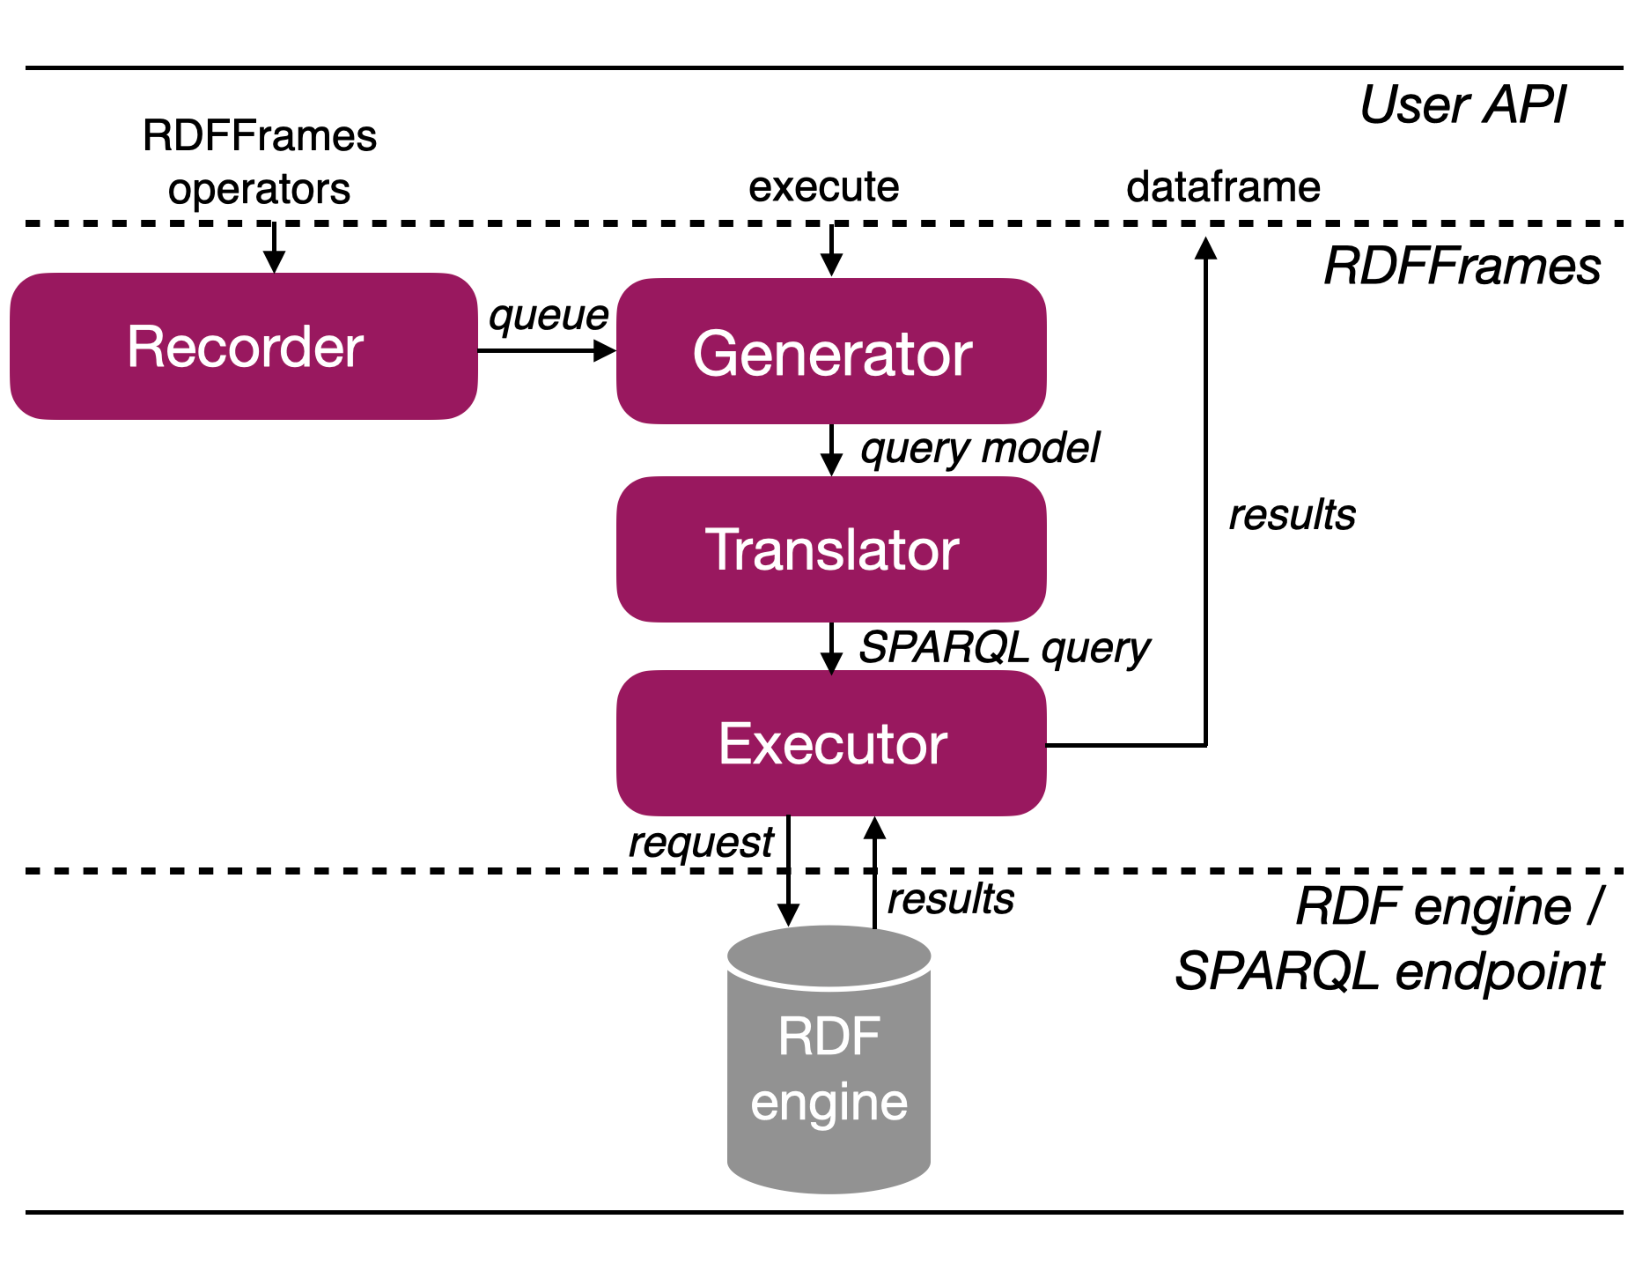
\includegraphics[width=0.8 \columnwidth]{figures/architecture}
  \caption{\rdfframes architecture.}
  \label{fig:architecture}
  \vspace*{-12pt}
\end{figure}


\noindent
\textbf{\rdfframes in a Nutshell.}
The architecture of \rdfframes is shown in Figure~\ref{fig:architecture}.
At the top of the figure is the user API, which consists of a set of operators implemented as Python functions.
We make a design decision in \rdfframes to use a \textit{lazy evaluation strategy}.
Thus, the \texttt{Recorder} records the operators invoked by the user without executing them,
storing the operators in a FIFO queue.
The special \texttt{execute} operator causes the 
\texttt{Generator} to consume the operators in the queue and build a {\em query model} representing the user's code.
The query model is an intermediate representation for
%that resembles a 
\sparql queries. The goal of the query model is (i)~to separate the API parsing logic from the query building logic for flexible manipulation and implementation, and (ii)~to facilitate optimization techniques for building the queries, especially in the case of nested queries.
Next, the \texttt{Translator} translates the query model into a \sparql query.
This process includes validation to ensure that the generated query has valid \sparql syntax and is equivalent to the user's API calls.
%This process includes validating the query model to ensure a valid \sparql syntax and its equivalence with the user's calls.
Our choice to use lazy evaluation means that the entire sequence of operators called by the user is captured in the query model processed by the \texttt{Translator}.
We design the \texttt{Translator} to take advantage of this fact and generate
\textit{compact and efficient} \sparql queries.
Specifically, each query model is translated to one \sparql query and the \texttt{Translator} minimizes the number of nested subqueries.
After the \texttt{Translator}, the \texttt{Executor} sends the
generated \sparql
query to an RDF engine or \sparql endpoint, handles all communication issues,
%the communication between the client and the RDF engine/endpoint,
and returns the results to the user in a dataframe.

\noindent

\textbf{Contributions:}
The novelty of \rdfframes lies in:
% three aspects:
\squishlist
\item
First, the API provided to the user is designed to be intuitive and flexible,
in addition to being expressive.
The API consists of navigational operators and data processing operators based on familiar relational algebra operations
such as filtering, grouping, and joins (Section~\ref{sec:data-model}).

\item
Second, \rdfframes translates the API calls into efficient \sparql queries.
A key element in this is the query model which exposes query equivalences in a simple way.
In generating the query model from a sequence of API calls and in generating the \sparql query from the query model,
\rdfframes has the overarching goal of generating efficient queries
(Section~\ref{sec:query-generation}).
We prove the correctness of the translation from API calls to \sparql. That is, we prove that the dataframe that \rdfframes returns is semantically equivalent to the results set of the generated \sparql query (Section~\ref{sec:correctness}).

\item
Third, \rdfframes handles all the mechanics of processing the \sparql query such as the connection to the RDF engine 
%database system 
or \sparql endpoint, pagination (i.e., retrieving the results in chunks) to avoid the endpoint timing out, and converting the result to a dataframe. 
We present case studies and performance comparisons that validate our design decisions
and
show that \rdfframes outperforms several
alternatives
%for accessing knowledge graphs from a machine learning software stack
%show that our query generation process outperforms simpler alternatives, and in 
(Section~\ref{sec:performance}).

\squishend

